\documentclass[border=0cm]{standalone}
\usepackage{tikz}

\begin{document}
\begin{tikzpicture}
    \node at (0,0)    {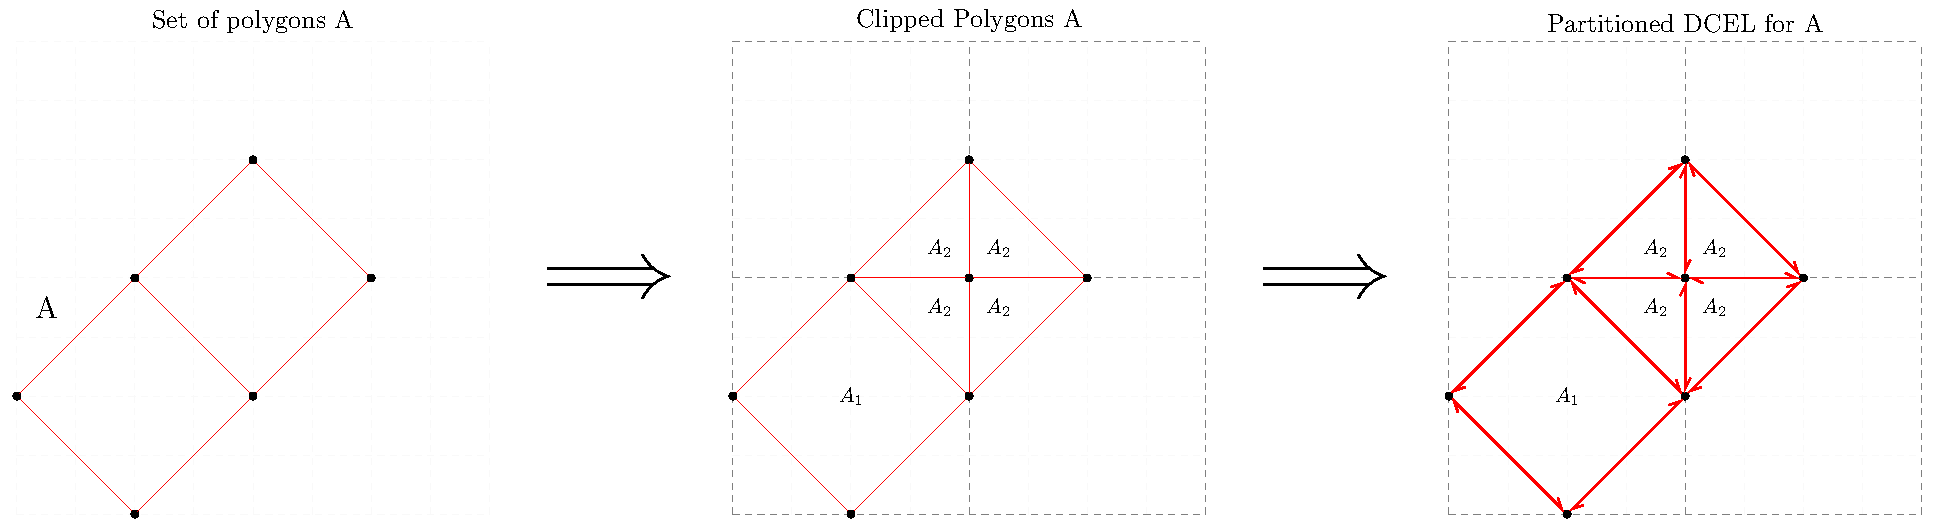
\includegraphics[scale=0.6]{PolygonAParted}};
    \node at (0,-5.5) {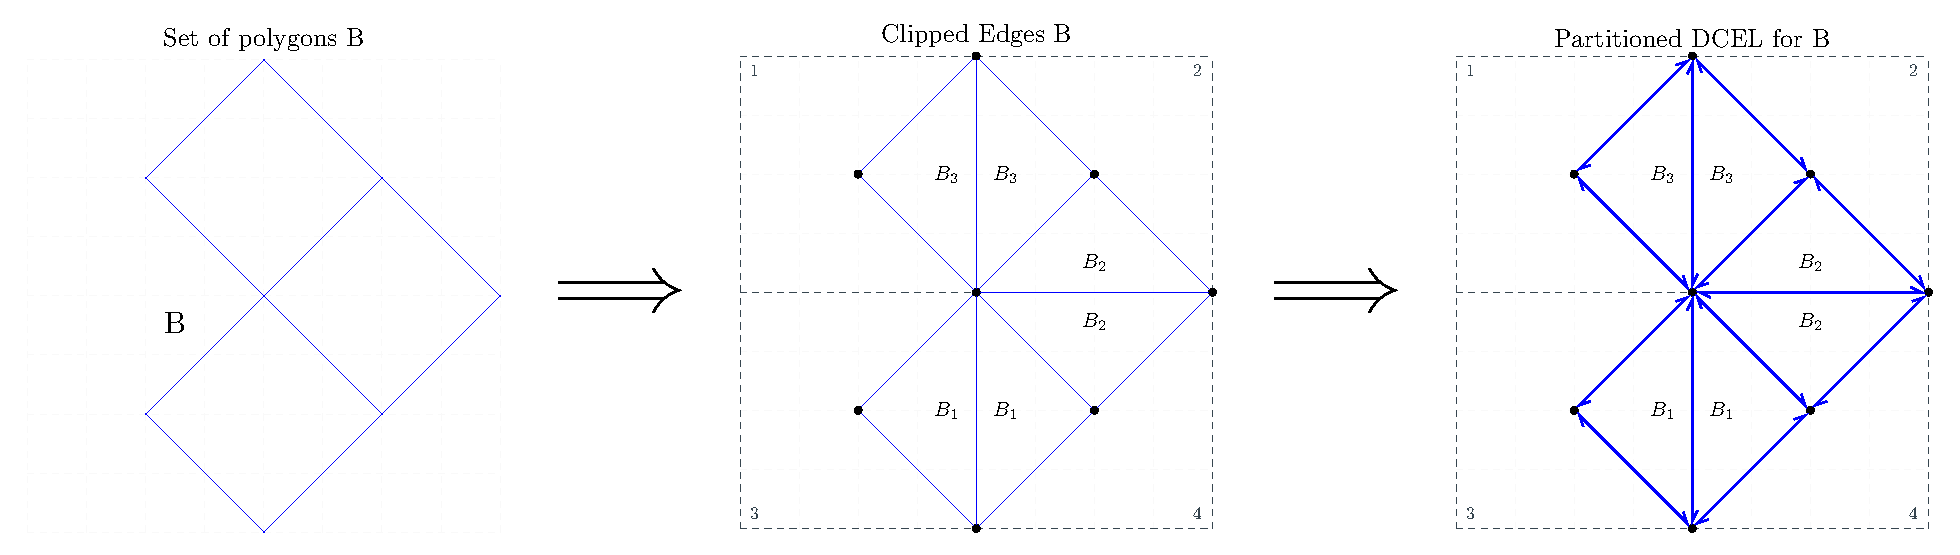
\includegraphics[scale=0.6]{PolygonBParted}};
    \node[rotate=-45, scale=2.5] at (11, -1.5)    {$\Longrightarrow$};
    \node[rotate=45,  scale=2.5] at (11, -5)    {$\Longrightarrow$};
    \node[scale=1] at (15, 0.3)    {Merge DCEL at partition level};
    \node at (15,-3)     {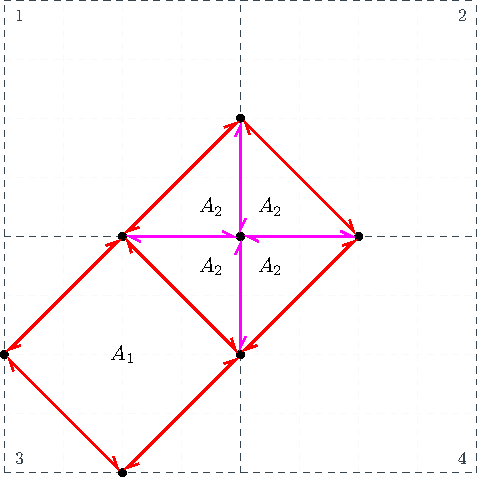
\includegraphics[scale=0.75]{MergePartsA}};
    \node at (15.4,-3.4) {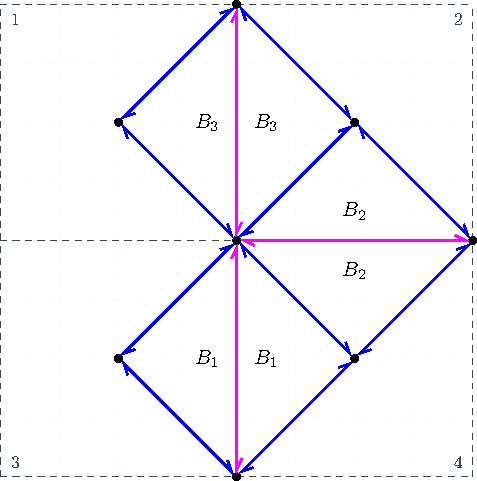
\includegraphics[scale=0.75]{MergePartsB}};
%    \node at (22,-3)     {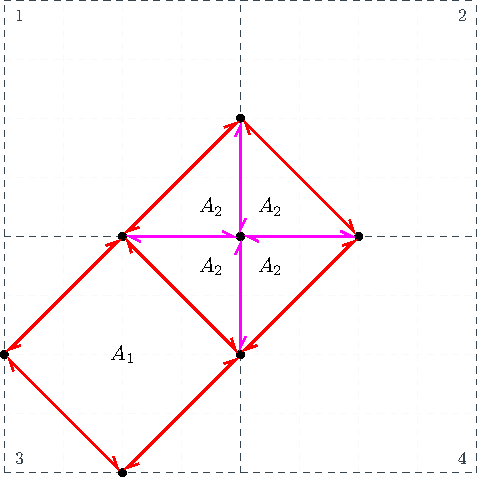
\includegraphics[scale=0.75]{MergePartsA}};
%    \node at (22.05,-2.98) {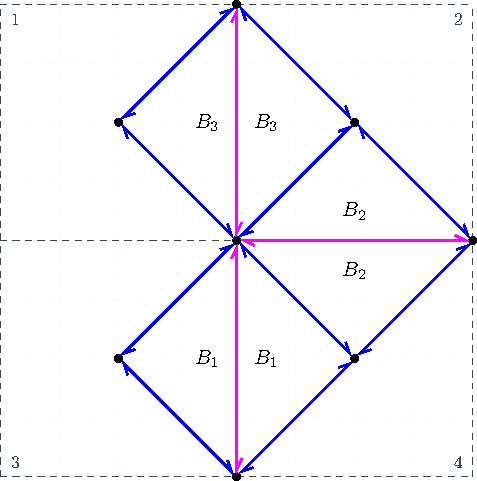
\includegraphics[scale=0.75]{MergePartsB}};
\end{tikzpicture}
\end{document}
